\documentclass[fleqn,usenatbib]{mnras}

\usepackage{newtxtext,newtxmath}
\usepackage[T1]{fontenc}
\DeclareRobustCommand{\VAN}[3]{#2}
\let\VANthebibliography\thebibliography
\def\thebibliography{\DeclareRobustCommand{\VAN}[3]{##3}\VANthebibliography}
\usepackage{graphicx}	% Including figure files
\usepackage{pict2e}
\usepackage{amsmath}	% Advanced maths commands
%\usepackage{amssymb}	% Extra maths symbols

%%%%%%%%%%%%%%%%%%%%%%%%%%%%%%%%%%%%%%%%%%%%%%%%%%

%%%%% AUTHORS - PLACE YOUR OWN COMMANDS HERE %%%%%

% Please keep new commands to a minimum, and use \newcommand not \def to avoid
% overwriting existing commands. Example:
%\newcommand{\pcm}{\,cm$^{-2}$}	% per cm-squared

%%%%%%%%%%%%%%%%%%%%%%%%%%%%%%%%%%%%%%%%%%%%%%%%%%

%%%%%%%%%%%%%%%%%%% TITLE PAGE %%%%%%%%%%%%%%%%%%%

% Title of the paper, and the short title which is used in the headers.
% Keep the title short and informative.
\title[Artificial Pulsar]{Tuning Low Frequency Pulsar Searching with an  Artificial Pulsar Device}

\author[J.-H. Gu et al.]{
Junhua Gu$^{1}$\thanks{E-mail: jhgu@nao.cas.cn} et al.
\\
% List of institutions
$^{1}$National Astronomical Observatories, Chinese Academy of Sciences, 20A Datun Road, Beijing, China
}
% These dates will be filled out by the publisher
\date{Accepted XXX. Received YYY; in original form ZZZ}

% Enter the current year, for the copyright statements etc.
\pubyear{2021}

% Don't change these lines
\begin{document}
\label{firstpage}
\pagerange{\pageref{firstpage}--\pageref{lastpage}}
\maketitle

% Abstract of the paper
\begin{abstract}
Abstract
\end{abstract}

% Select between one and six entries from the list of approved keywords.
% Don't make up new ones.
\begin{keywords}
keyword1 -- keyword2 -- keyword3
\end{keywords}

\section{Introduction}
\citet{2017AAS...22915516P}, \citet{2011AAS...21723406S}

\section{Artificial Pulsar Device}
The artificial pulsar device (APD hereafter) is a device that is able to emit simulated pulsar signal within some certain bandpass.
We design it to be able to simulate the dispersion effect and arbitrary pulse profile of a pulsar.
Our implementation of APD is composed of three modules: 1) a high performance workstation that is responsible of computing the pulsar signal online, 2) a software-defined radio (SDR) transmitter that accepts commands and data stream from the workstation and convert it to voltage signal, which is then fed into 3) a radio frequency front-end. 
The radio frequency front-end is further composed of a radio frequency power amplifier (PA hereafter) and an antenna that is used to broadcast the actual signal.

\begin{figure}
    \centering
    \includegraphics[width=0.95\columnwidth]{flow_chart.pdf}
    \caption{The flow chart of emitting the simulated pulsar signal.
    }
    \label{fig:flow_chart}
\end{figure}


The APD can be placed near the low-frequency pulsar observation device (LFPOD hereafter). 
Though possible, it is not necessary for the emitting antenna to be placed inside the range of the primary beam LFPOD.
The power of the emitted signal can be amplified to a high enough level so that when the signal is received by the LFPOD from its side lobes it approximates the power level of a natural pulsar.

In this section, we describe the algorithms and steps that are used to generate the radio frequency signal, which is later used to tune LFPODs.

\subsection{Important Approximations that We Make}
The purpose of this work is to present a method of tuning the search of pulsars in low frequency radio band, which is composed of signal receiving/recording and signal detection.
Dedispersion is an important step in the signal detection stage.
According to e.g., \citet{2012hpa..book.....L}, it is possible to perform either coherent dedispersion or incoherent dedispersion. The former works on raw baseband data and the latter works on channelized filterbank data. 
The main different between these two category of dedispersion methods is whether phase information is kept in the input data.
In order to enable the generated signal suitable to both category of dedispersion methods, we have to ensure that the phase information is treated with caution.
Considering that fact that the dispersion caused by ISM can cause delays of different frequencies in low frequency band to reach at most $10^2$ s time scale, computing the dispersed pulsar signal online without necessary approximation is infeasible.

We make following approximation when generating the artificial pulsar signal: the pulsar signal (not only the amplitude profile, but also the signal phase) repeats with a period of $n\tau$, where $\tau$ is the period of the pulsar, $n$ is an integer. The value of $n$ is chosen so that it is affordable by the computation resource of the workstation that we use to generate the signal and large enough to ensure good enough statistics in folding. 
With above approximation the frequency components contained in the signal become discrete so that the phase delays of all the frequency components can be computed precisely.

In practice, we choose the value of $n\tau$ around $1$ s.
As the signal can be computed offline, this value can reach several seconds to dozens of seconds.
If incoherent dedispersion method is used, it is also possible to update the repeating signal samples every tens of seconds (this time interval is determined by computing performance), for the phase information is not important. 


\subsection{Computing Artificial Pulsar Signal}
\subsubsection{Generating baseband I/Q samples}
The pulse amplitude profile $f(\theta)$, where $\theta$ is the pulse phase should meet following constraint
\begin{gather}
    f(\theta+1)=f(\theta).
\end{gather}
In following sections we utilize a Gaussian function with a pulse width parameter $w$ to describe the profile:
\begin{gather}
    f(\theta)=\left \{
    \begin{array}{rl}
        f(\theta-1) &\theta \geq 0.5\\
         \exp(-\frac{\theta^2}{2w^2}) & \theta\in[-0.5, 0.5) \\
        f(\theta+1) &\theta < -0.5\\
    \end{array}
    \right ..
\end{gather}
Assuming a frequency range of $[\nu_{\min}, \nu_{\max}]$, the sampling interval $dt$ is also fixed as $dt=1/B$, where $B=\nu_{\max}-\nu_{\min}$.
Thus the baseband I/Q sample series is generated as 
\begin{gather}
    y_j=f(\frac{j\times dt}{\tau})\frac{x^{\rm re}_j+x^{\rm im}_ji}{2}, j=1..\left \lfloor\frac{n\tau}{dt} \right\rfloor
\end{gather}
where each $x^{\rm re}$'s and $x^{\rm im}$'s independently follows a standard normal distribution. 


 \subsubsection{Applying the dispersion effect}
  Applying the ISM dispersion effect is simply an inverse operation of coherent dedispersion with some slight differences.
  According to e.g., \citet{2012hpa..book.....L}, we calculate the dispersed baseband I/Q sample series as
  \begin{gather}
      \mathbf{y}^d={\rm IDFT}(\mathbf{Y}^d)
  \end{gather}
  \begin{gather}
      Y_j^d={\rm DFT}(\mathbf{y})_j\exp(2\pi i \nu_j\Delta t(\nu_j)),
  \end{gather}
  where ${\rm DFT}$ and ${\rm IDFT}$ denote the forward and backward discrete Fourier transform, respectively, $\mathbf{y}$ is a vector with each of its element to be $y_j$, $\mathbf{Y}$ is a vector with each of its element to be $\mathbf{Y}_j$, $\nu_j$ is the frequency corresponding to the $j$-th frequency channel, and the delay cause by the dispersion is calculated as 
  \begin{gather}
     \Delta t(\nu)\simeq 4.15\times 10^6~{\rm ms}~\left(\frac{{\rm MHz}}{\nu}\right)^2\frac{\rm DM}{\rm pc~cm^{-3}},
 \end{gather}
 according to e.g., \citet{2012hpa..book.....L}.
 
 

 \begin{figure}
    \centering
    \includegraphics[width=0.9\columnwidth]{dm1_profile.pdf}
    \caption{Frequency dependent pulse profile with a $\rm DM=1$ pc cm$^{-3}$ dispersion effect applied. The parameter of the pulsar
    is same as the one used in Figure \ref{fig:dm0_profile}}
    \label{fig:dm1_profile}
 \end{figure}

\subsubsection{Generating the narrow band I/Q sampling data}
 
With the amplitude profile in hand, we go on to generate the narrow band in-phase and quadrature (I/Q hereafter) signals.
First we determine the sampling interval $dt$ of the final generated I/Q time series signal and the number of frequency channels to $N_{\rm ch}$ be used in follow up procession.
The number of frequency channels further determines the bandwidth of each frequey channel as
\begin{gather}
    d\nu=\frac{f_{\max}-f_{\min}}{N_{\rm ch}}.
\end{gather}
For the sampling interval $dt$, according to the Nyquist Theorem the upper limit of which has to be $\frac{1}{2BW}$. 
For we are using I/Q sampling here the upper limit of the sampling interval is enlarged to $1/BW$.
The sampling interval of the narrow band I/Q data for current step can be calculated as
\begin{gather}
 dT=\frac{dt}{2N_{\rm ch}}.
\end{gather}
The factor 2 in the denominator is oversampling factor that we choose.
Thus the number of time bins within each period is determined 
\begin{gather}
 N_{\rm t}=\left\lfloor\frac{\tau}{dT}\right\rfloor.
\end{gather}
Note that in order to achieve a high computing performance, we limit the actual period $\tau$ can only be an integer multiple of $dT$.

So that for each frequency bin and time bin in a single period, we can calculate its instant complex voltage as
\begin{gather}
    U(\nu_{j}, t_{k})=\frac{1}{2}f^{\rm d}(\nu_j, t_{k}/\tau)(x^{\rm re}(j,k)+x^{\rm im}(j,k)i),
\end{gather}
where $j=1..N_{\rm ch}$, $k=1..N_{t}$, $i^2=-1$, and each $x^{\rm re}$ and $x^{\rm re}$ follows a standard normal distribution $\mathcal{N}(0,1)$ independently.

\subsubsection{Generating baseband I/Q sampling data stream}

The narrow band I/Q data is then fed into a over-sampled polyphase filterbank (PFB) to synthesize a broadband base-band I/Q data stream.
We take the work of \citet{2020JAI.....950004M} as a reference of designing the PFB.
We set the number of channels to be $N_{\rm ch}=16384$ and the taps of each channel to be 12.
PFBs are a kind of standard digital signal processing steps, so we just skip the details of the PFB that we use in this work.

The PFB outputs the baseband I/Q sampling time series.
We plot a sample of the baseband I/Q sample data in Figure \ref{fig:iq_data}(a), the DM of which is $1$ pc cm$^{-3}$.
It is obvious that all apparent time domain feature has been smeared because of the dispersion, so that pure time domain analysis is hardly possible to detect the fake pulsar we simulated here.
As a comparison, we present the same plot of the I/Q data with DM=0 pc cm$^{-3}$ in Figure \ref{fig:iq_data}(b), in which pulse-like time domain structure can be recognized clearly.
The I/Q sampling data stream is then sent to an SDR transmitter so that actual radio frequency (RF) signal within desired frequency range is generated continuously.
The RF signal is fed into a power amplifier and broadcast through a proper antenna. 

\begin{figure}
    \centering
    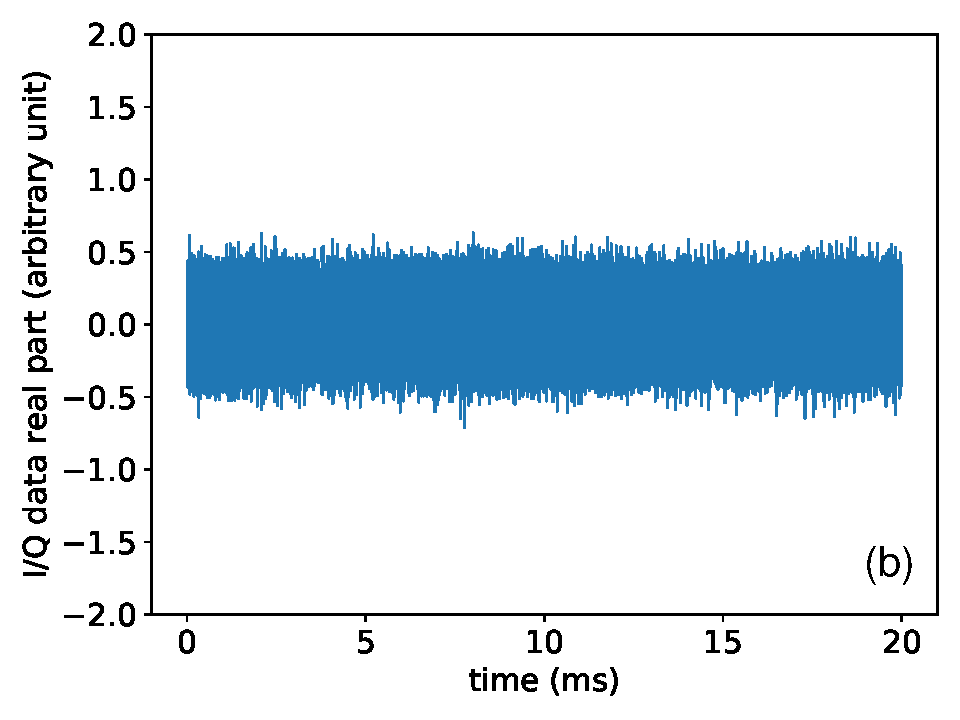
\includegraphics[width=0.95\columnwidth]{dm1_iq.pdf}\\
    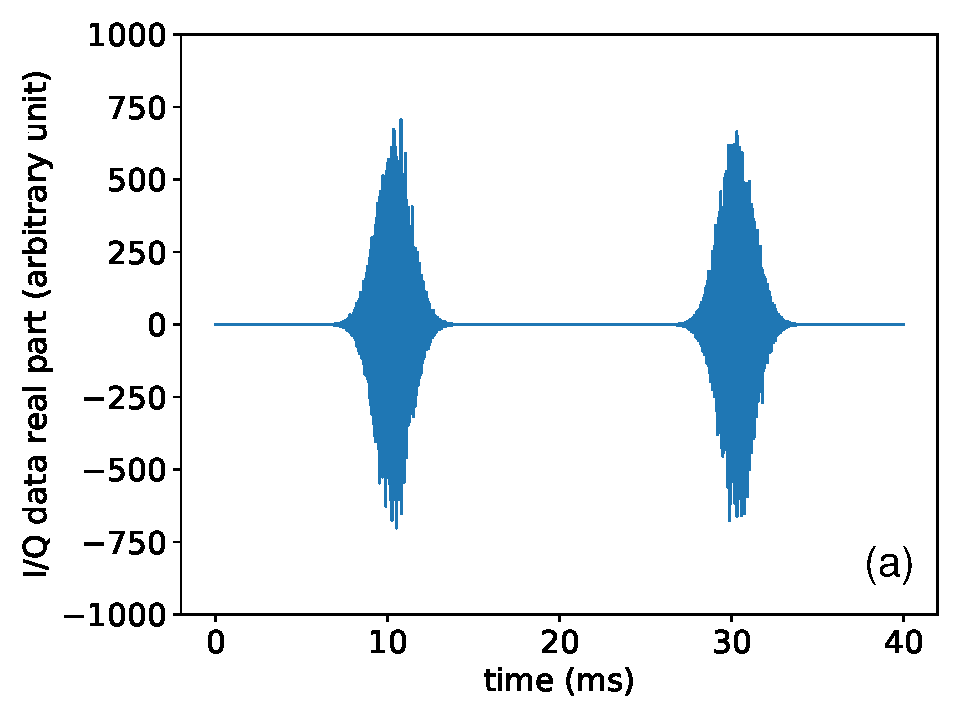
\includegraphics[width=0.95\columnwidth]{dm0_iq.pdf}
    \caption{The real part of the baseband I/Q data as a function of time. Two periods are shown here. The period is set to be 20 ms, in (a) the DM is set to be 10 pc cm$^{-3}$ and in (b), the DM is set to be 0 pc cm$^{-3}$ for the purpose of comparison.}
    \label{fig:iq_data}
\end{figure}

\subsection{Emitting Generated Signal}

\section{An Example of Tuning}

\section{Discussion}

\section{Conclusions}

\section*{Acknowledgements}


%%%%%%%%%%%%%%%%%%%%%%%%%%%%%%%%%%%%%%%%%%%%%%%%%%

\bibliographystyle{mnras}
\bibliography{ms}

%%%%%%%%%%%%%%%%%%%%%%%%%%%%%%%%%%%%%%%%%%%%%%%%%%


% Don't change these lines
\bsp	% typesetting comment
\label{lastpage}
\end{document}

% End of ms.tex
